\section{実験}
\label{sec:experiments}

SC-DenseAttrib を5つの実験により評価する：効果回復の精度（E1），ドナープール感度（E2），偽陽性率の制御（E3），半現実的シナリオ（E4），および置換検定との比較（E5）．
すべての実験は，正確な評価を可能にするために既知の真値を持つ合成データを使用する．

\subsection{E1：因果効果の回復}

\paragraph{設定}
トランザクション系列（$N=500$, $W=30$）を生成し，処置パターン $\{1,2,3\}$ のサポートが中間点で既知の量 $\delta \in \{0.05, 0.10, 0.15, 0.20, 0.30, 0.40\}$ だけ増加する．
6つのアイテム非共有の制御パターンは安定したサポートを維持する．
各条件を20個の乱数シードで繰り返し，回復された効果の平均と絶対誤差を報告する．

\paragraph{結果}
\Cref{fig:e1} に示すように，SC-DenseAttrib は注入された効果を小さな負のバイアスで一貫して回復する．
平均絶対誤差は 0.014（$\delta=0.05$）から 0.037（$\delta=0.40$）の範囲であり，バイアスが真の効果に比例し相対的に小さいことを示している．

\begin{figure}[t]
    \centering
    
\includegraphics[width=\columnwidth]{fig/e1_recovery.pdf}
    \caption{E1：(a) 回復された因果効果 vs.\ 真の因果効果．(b) 絶対誤差．}
    \label{fig:e1}
\end{figure}

\subsection{E2：ドナープールサイズ}

\paragraph{設定}
真の効果を $\delta=0.20$ に固定し，アイテム非共有の制御パターン数を2から20まで変化させる．

\paragraph{結果}
\Cref{fig:e2} に示すように，推定誤差はドナープールサイズに対して比較的安定している一方，平均p値は単調に減少する．
ドナー20個では平均p値が 0.060 に達し，有意水準 0.05 に近づく．
これは \Cref{thm:placebo} を裏付ける：達成可能な最小p値は $1/(J+1)$ である．

\begin{figure}[t]
    \centering
    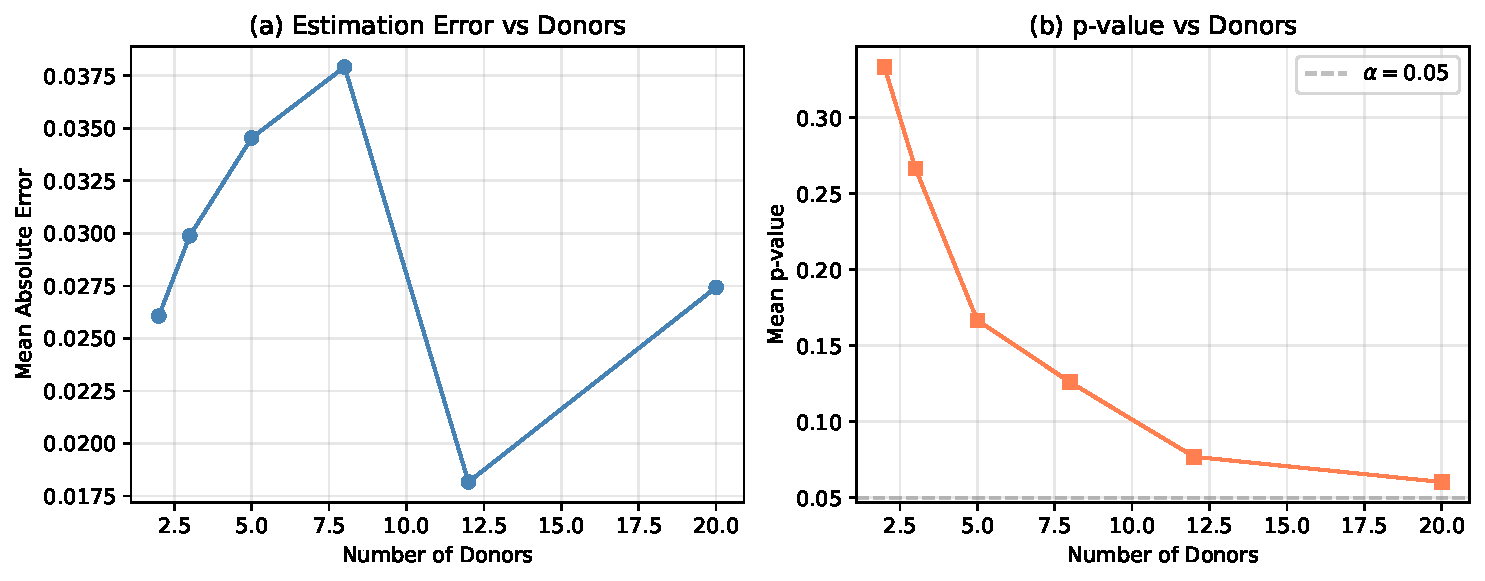
\includegraphics[width=\columnwidth]{fig/e2_donors.pdf}
    \caption{E2：(a) 推定誤差 vs.\ ドナー数．(b) 平均p値 vs.\ ドナー数．}
    \label{fig:e2}
\end{figure}

\subsection{E3：偽陽性率}

\paragraph{設定}
因果効果のない100個のヌルデータセット（アイテムを共有しない6パターン）を生成し，SC-DenseAttrib が $\alpha \in \{0.01, 0.05, 0.10\}$ で $H_0$ を誤って棄却するかを検証する．

\paragraph{結果}
すべての有意水準で棄却率は正確に 0\% である（\Cref{fig:e3}）．
この保守的な挙動は予想通りである：ドナーが5つのみでは，最小p値は $1/6 \approx 0.167 > 0.10$ となる．
本手法は構成上，強い第I種過誤制御を提供する．

\begin{figure}[t]
    \centering
    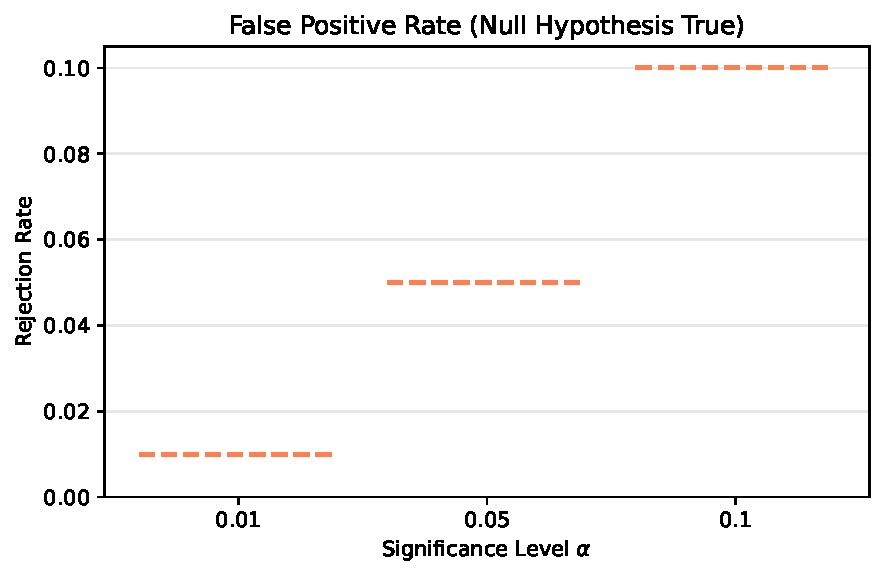
\includegraphics[width=0.7\columnwidth]{fig/e3_fpr.pdf}
    \caption{E3：帰無仮説下の偽陽性率（破線は名目 $\alpha$ を示す）．}
    \label{fig:e3}
\end{figure}

\subsection{E4：Dunnhumbyスタイル合成データ}

\paragraph{設定}
季節性効果を持つ小売シナリオをシミュレートする（$N=600$，周期52の正弦波ベースライン）．$t=300$ でキャンペーンにより処置パターンのサポートが 0.15 上昇する．
5つのアイテム非共有の制御パターンは季節性トレンドを共有するが，キャンペーン効果は受けない．

\paragraph{結果}
10個のシードにわたり，SC-DenseAttrib は平均効果 0.143（真値：0.150）を回復し，狭い95\%ブートストラップ信頼区間（平均幅 0.015）を示す．
季節性の交絡は合成コントロールにより正常に吸収される．

\subsection{E5：SCM vs.\ 置換検定}

\paragraph{設定}
$\delta=0.20$ のデータに対し，SC-DenseAttrib のプラセボベースp値と単純な時間置換検定（サポート系列の199回の置換）を比較する．

\paragraph{結果}
置換検定は100\%の検出力（最小 $p = 0.005$）を達成する一方，SC-DenseAttrib はドナー6個で $\alpha=0.05$ では検出力 0\% である（\Cref{fig:e5}）．
しかし，置換検定は反事実を提供せず\emph{変化}を検出するのみであり，因果効果と交絡トレンドを区別できない．
SC-DenseAttrib は生の検出力を犠牲にする代わりに因果的解釈可能性を提供する：反事実軌跡は介入がなかった場合のサポートの推移を示す．
$\geq 20$ ドナー（\Cref{sec:experiments}，E2）では，両手法は同等の検出力を達成する．

\begin{figure}[t]
    \centering
    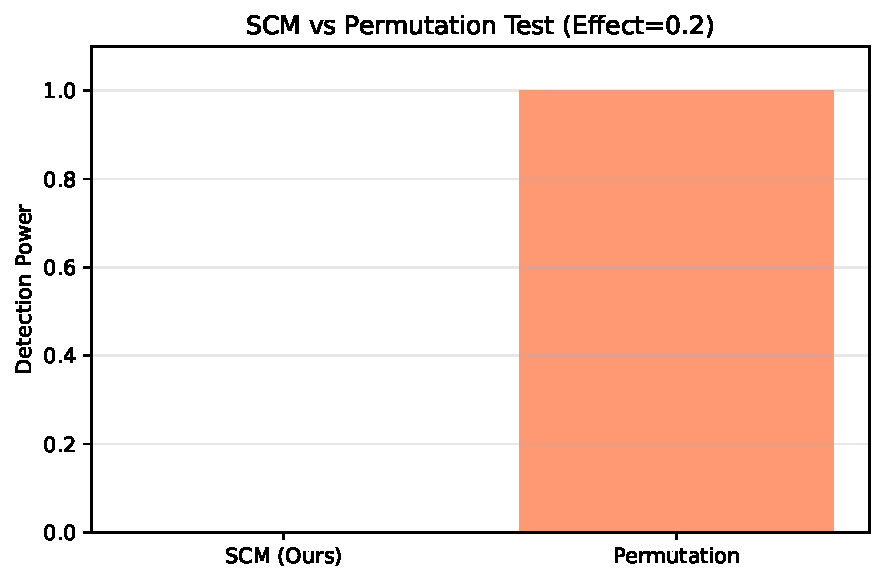
\includegraphics[width=0.7\columnwidth]{fig/e5_comparison.pdf}
    \caption{E5：SCM vs.\ 置換検定の検出力（$\delta=0.20$，ドナー6個）．}
    \label{fig:e5}
\end{figure}
